%%%
%%% Copyright (c) 2010 Jens Haase <je.haase@googlemail.com>
%%%
%%% Permission is hereby granted, free of charge, to any person obtaining a copy
%%% of this software and associated documentation files (the "Software"), to deal
%%% in the Software without restriction, including without limitation the rights
%%% to use, copy, modify, merge, publish, distribute, sublicense, and/or sell
%%% copies of the Software, and to permit persons to whom the Software is
%%% furnished to do so, subject to the following conditions:
%%%
%%% The above copyright notice and this permission notice shall be included in
%%% all copies or substantial portions of the Software.
%%%
%%% THE SOFTWARE IS PROVIDED "AS IS", WITHOUT WARRANTY OF ANY KIND, EXPRESS OR
%%% IMPLIED, INCLUDING BUT NOT LIMITED TO THE WARRANTIES OF MERCHANTABILITY,
%%% FITNESS FOR A PARTICULAR PURPOSE AND NONINFRINGEMENT. IN NO EVENT SHALL THE
%%% AUTHORS OR COPYRIGHT HOLDERS BE LIABLE FOR ANY CLAIM, DAMAGES OR OTHER
%%% LIABILITY, WHETHER IN AN ACTION OF CONTRACT, TORT OR OTHERWISE, ARISING FROM,
%%% OUT OF OR IN CONNECTION WITH THE SOFTWARE OR THE USE OR OTHER DEALINGS IN
%%% THE SOFTWARE.
%%%

\documentclass[11pt, accentcolor=tud9b, nochapname]{tudreport}

\usepackage[utf8]{inputenc}
\usepackage[english]{babel}
% \usepackage{fontenc}
% \usepackage{graphicx}
\usepackage{url}
\usepackage{cite}
\usepackage{longtable}
\usepackage{listings}
% \usepackage{wrapfig}
% \usepackage[numbers]{natbib}

\begin{document}

\author{Jens Haase}
\title{Analyzing German Noun Compounds using a
  Web-Scale Dataset}
\subtitle{UIMA Software Project WS 2010/2011}
\subsubtitle{Jens Haase}
\date{\today}
\maketitle

\begin{abstract}
Noun-compounding in the German language is a tool to combine two or more single words to new words. In information retrieval and search engines this can be a problem because mostly documents with the combined and the splitted words are relevant for a search query. To get better search results it is often required to split words into single parts.
\end{abstract}

\setcounter{tocdepth}{3}
\tableofcontents

\chapter{Introduction}

\section{Motivation}
Noun-compounding in the German language is a powerful process to build
new words with the combination of two or more existing
words. \emph{Blumensträuße} (flower bouquet) for example contains the
two words \emph{Blumen} (flower) and \emph{Sträuße} (bouquet).

In Unstructured Information Management this can be a handicap for
tools like Machine Translation, Speech Recognition or Information
Retrieval. Imagine you search for the word \emph{Lackschicht} (paint
layer), the expected result will be all documents containing the word
\emph{Lackschicht} but also the words \emph{Schicht aus Lack} (layer of
paint). To find a expected result the search engine must split all
compounds nouns in single words (\emph{Lackschicht} -> \emph{Lack schicht}).

\section{Problem definition}
In the German language a compounds can be formed by combining nouns,
verbs and adjectives. Also compound words can combined to a new
compound word. The word \emph{Donaudampfschifffahrtskapitänsmütze} (a
cap for captains of steamboats driven on the river Donau), contains the
words \emph{Donaudampfschiff} (steamboat on the river Donau) and
\emph{Kapitänsmütze} (the cap of the captain). Each word can be
split again. The final decompounds words are \emph{Donau},
\emph{Dampf}, \emph{Schiff}, \emph{Fahrt}, \emph{Kapitän} and
\emph{Mütze}.

Another problem in noun decompounds are linking morphemes. These
morphemes are allowed between two words. The linking morpheme in
\emph{Kaptiänsmütze} is the the \emph{s} between \emph{Kapitän} and
\emph{Mütze} (\emph{Kapitän(s)+mütze}). Also the word
\emph{Orangensaft} (orange juice) has a \emph{n} as linking morpheme
(\emph{Orange(n)+saft)}. But in this case the word \emph{Orangen} is a
valid word in the German language. It is the plural of the word
\emph{Orange}. But the word \emph{Kapitäns} in previous example is not
a valid word.

At least not all possible splits have the same meaning. The word
\emph{Tagesration} (recommended daily amount), contains the word
\emph{Tag} (day), \emph{Rat} (advice) and \emph{Ion} (ion) but also
the word \emph{Ration} (ration). Splitting the the word in three
parts is wrong, because the chemical ion has nothing to do with the
word \emph{Tagesration}. The correct decompounding here will be
\emph{Tag(es)+ration}.

\section{Task description}
Decompounding of a word is mostly done in three steps \cite{alf2008}:

\begin{enumerate}
\item[1.] Calculate every possible way of splitting a word in one or more
  parts
\item[2.] Score those parts according to some weighting function
\item[3.] Take the highest-scoring decomposition. If it contains one part,
  it means that the word in not a compound.
\end{enumerate}

At first we have to split a word in all possible parts. For that we
need a dictionary with all existing words. It is recommend to use a
special dictionary for the analyzing corpus. This can simple be done
in extracting all tokens of a document collection. A list of linking
morphemes is also needed.

In the next step we need a weighting function for each decompound
possibility. The can be for example a simple count frequency of every
word. The words with more frequency get a higher weight than other. At
the end we can rank the weights. The decomposition with the highest
weight wins.

At the end we want to have UIMA component that can be used in other
projects. It should able to work with special dictionaries and linking
morphemes. Optional different weighting function can be chosen.

\chapter{How to split a word}

\section{Helpful Tools}

\subsection{IGerman98 Dictionary}
As mentioned early it is recommend to build a dictionary for a special
corpus, but in this case we do not have a special corpus. Instead we
want to use a \emph{every day} dictionary, which are used for spell
correction. ASpell and ispell are open source spell checker with
dictionaries for nearly every language. Also hunspell is a modern
spell checker, used in OpenOffice, Mozilla Firefox and Google
Chrome.

The dictionary used in these tools is mostly the \emph{IGerman98}
dictionary from Björn Jacke. Different versions can be found
on his website \url{http://www.j3e.de/ispell/igerman98/}.

The dictionary contains of two different files. A word list
and a rule set. With the rule set the affixes (suffix and/or prefix)
of a word can be changed.

\subsection{Google Web1t and Lucene}
Google Web1T corpus contains over 130 billion tokens of the German
language, distributed over n-grams ($n \epsilon [1,5]$). The corpus
is used for different ranking function.

The corpus itself provides no access or search tools. For that a index must be
created. The most common tool for full text search today
is Lucene. This will be used to create a index of the
corpus and provided a search function.

Another tool to access the the data is the \emph{jWeb1T}
(\url{http://hlt.fbk.eu/en/technology/jWeb1t}) tool. This
was not used because it can only check if a given n-gram
is contained in the corpus.

\subsection{Evaluation corpus}
For the evaluate the result of the work the corpus of Marek
\cite{marek} was used. The corpus was semi-automatically
created and contains over 160,000 examples.

The corpus can be found in the code resources or on Marek'
website \url{http://diotavelli.net/files/ccorpus.txt}

\subsection{CouchDB and Javascript}
To visualize the splitting algorithm CouchDB and Javascript
are used. CouchDB (\url{http://couchdb.apache.org/}) is an document data store, which stores JSON data. The complete database is accessible via a HTTP interface. Next to the JSON data a document can also have attachments. These can be used to serve a little application to the browser.

With some Javascript it is possible to write a complete application
without a middleware between the client and the database. Together with
Javascript InfoVis Toolkit \url{http://thejit.org} it is very
easy to visualize the splitting algorithm in a browser.

\subsection{UimaFit}
At the end of the project a complete UIMA \url{http://uima.apache.org/} component should be implemented to use the work in further projects. UIMA is an framework for unstructured information management systems. With the framework components can be implements and reused in different applications.

UimaFit \url{http://code.google.com/p/uimafit/} is build on top of UIMA to make development in UIMA easier, faster and more flexible. The library provides factories, injection and testing utilities.

\section{Implementation}

\subsection{Prerequirements}

\subsubsection{Dictionary access}
The simplest form of a dictionary is a list of words. This is what the \texttt{SimpleDictionary} class can do. It gets a filename as parameter and uses each line in this file as a word of the dictionary. This class can be easily used for your own special dictionary. For example if you export a dictionary from a large dataset.

For the rest of this work we used the popular IGerman98 dictionary from Björn Jacke. This dictionary consist of two parts. The first part is a list of annotated words. These are the base words of the dictionary. The second part is rule set that changes the base word in it's prefixes and suffixes. For example the following dictionary file contains three words; two of them are annotated (word and annotation are separated by a slash).

\begin{lstlisting}
hello
try/B
work/AB
\end{lstlisting}

The rule set describes the annotation. \texttt{PFX} stands for Prefix and \texttt{SFX} for suffix. In the following files you see a prefix rule for \texttt{A} and a suffix rule for \texttt{B}:

\begin{lstlisting}
PFX A Y 1
PFX A 0 re .

SFX B Y 2
SFX B 0 ed [\^y]
SFX B y ied y
\end{lstlisting}

Using this rules on the base words leads to new words. In this example we end up with six different words:

\begin{lstlisting}
hello
try
tried
work
worked
rework
\end{lstlisting}

The rule set also allows the combination of suffix rules and affix rules. But in the current implementation of the \texttt{IGerman98Dictionary} this is not handled. If you want to create your own dictionary implementation just implement the \texttt{IDictionary} interface in your code.

As mentioned above for all further work the \emph{IGerman98} dictionary is used. It currently contains 326,207 words. Without using the rule set the dictionary has only 81,612 words.

\subsubsection{Google Web1T Lucene index}
The ranking of the different split should be done with the Google Web1T dataset. The German dataset has a compressed file size from around 3.0 GB. The extracted files result in many text file, each containing a sorted list of n-grams. The following listing shows the file format of one row.

\begin{lstlisting}
  token-1 <space> ... <space> token-n <tab> frequency
\end{lstlisting}

Example:

\begin{lstlisting}
relax                150
relax on the couch   100
working is hard      200
\end{lstlisting}

While the compressed size of the German corpus is 3 GB, the extracted
files have a size of 11,3 GB and contain following data:

\vspace{10pt}
\begin{tabular}{| l | l |}
  \hline
  Number of tokens: & 131,435,672,897 \\ \hline
  Number of sentences: & 15,715,470,319 \\ \hline
  Number of unigrams: & 15,133,396 \\ \hline
  Number of bigrams: & 88,668,144 \\ \hline
  Number of trigrams: & 154,226,178 \\ \hline
  Number of fourgrams: & 140,670,210 \\ \hline
  Number of fivegrams: & 100,542,274 \\ \hline
  Number of n-grams: & 499,240,202 \\ \hline
\end{tabular}
\vspace{10pt}

The first plan to access the data in Java was to use the jWeb1T tool
(\url{http://hlt.fbk.eu/en/node/81}). This tool can find n-grams in a
logarithmic time. But it can only find the frequency for a given
n-gram. For example if the n-gram 'hello world' is listed in the
corpus with the frequency 50, the jWeb1T tool will find the n-gram by
searching for 'hello world', but not by searching for 'hello' or
'world'.

The ranking function should search for 'hello' and get all
n-grams containing the word 'hello'. When it searches for 'hello world' it
want to find the all n-grams with the words 'hello' and 'world'.

A second tool is the Java API for Web-1T Corpus of Digital Pebble
\url{http://www.digitalpebble.com/resources.html}. The tool is
currently not free available, but it is possible to contact Digital
Pebble. According to Julien Nioche of Digital Pebble the tool is
comparable to jWeb1T, but they are currently working on a new version
that will be freely available soon. Since there was no time to wait
for this tool we have to create our own indexer.

To index all n-grams Lucene was used. Each Lucene document contains a n-gram and the frequency. That means we do not need the extracted Web1T file for the next steps anymore. Creating the index is done with \texttt{LuceneIndexer} class. but for your own generation you can use the command line tool under \texttt{bin/web1TLuceneIndexer}. It comes with the following options:

\begin{lstlisting}
usage: LuceneIndexer
    --web1t <arg>        Folder with the web1t extracted documents
    --outputPath <arg>   File, where the index should be created
    --igerman98          (optional) If this argument is set, only words of
                         the german dictionary will be added to the index
    --index <arg>        (optional) Number of how many indexes should be
                         created. Default: 1
\end{lstlisting}

First you have to set the folder were all extracted text files of the web1t corpus are listed (\texttt{--web1t}). With the \texttt{outputPath} parameter you can specify were the index should be created on your disk. When you set the \texttt{igerman98} parameter only n-gram with words that are in the dictionary will be added to the index. For example if the dictionary contains the words \emph{Blumen} and \emph{Orange}, n-grams like \emph{Blumen sind schön} and \emph{Orangen sind orange} will be added but \emph{Hallo Welt} will be ignored. With this parameter you can reduce the size off the index on your disk. At least, with the \emph{index} parameter you can split the index in several independent indexes. Lucene can only store \texttt{Integer.MAX\_VALUE} number of documents per index. If you have a larger index you can use this option to split the index. Splitting the index to improve the speed will only work if the indexes run on different machines.

To access and search on the generated index the \texttt{Finder} class can be used. This class also detects splitted indexes in you put them in the same folder. To search for n-grams use the \texttt{find} function in the \texttt{Finder} class. This function returns a list of n-gram. Each n-grams contains the text and the frequency.

The generation of the index takes, depending on your hardware, a lot of time. On my machine the generation of the index takes about five hours. Writing to Solid State Disk or RAM can decrease the generation time. At the end, the index has a size of 23.4 GB without the \texttt{igerman} parameter. With the \texttt{igerman98} parameter the index is only 12.8 GB big.

With a normal hard disk and such a great index the queries are very slow. Most of the time they take about one seconds. This was also a problem for the evaluation. The evaluation of the complete corpus takes several days. For that only on a small amount of 10,000 examples the ranking algorithm were evaluated. To improve the query speed better hardware is need. It is highly recommended to put the index in a RAM. Also an other index mechanism can help to improve the speed.

The corpus used to evaluate the ranking function was generated with following command:

\begin{lstlisting}
./bin/web1TLuceneIndexer \
  --web1t /path/to/web1t/folder \
  --outputPath /path/to/generated/index \
  --igerman98
\end{lstlisting}

\subsubsection{Corpus reader}

For the evaluation of the algorithm the corpus of Marek \cite{marek} is used. The corpus was generated semi-automatic and contains 158,653 examples. Each line in the file contains a word and the correct split for the word. Splits are marked with \texttt{+} between individual parts. Each part also contains a annotation like \texttt{PREP, A, N, ...}. Morphemes are separated with a \texttt{|} or brackets. The following listing shows some examples.

\begin{lstlisting}
zugangsliste zu{PREP}+gang|s{A,N}+liste{N}
fachkameras fach{V,N}+kamera(s){N}
doppelprozessormaschine doppel{N,V}+prozessor{N}+maschine{N}
filmtauscher film{N,V}+tauscher{N}
minimalanforderungen minimal{A}+anforderung(en){N}
berufungsinstanz berufung|s{N}+instanz{N}
bleistiftstriche blei{N}+stift{N,V}+strich(e){N}
fernmeldeunion fern{A}+meld|e{V}+union{N}
ortsnetzmonopol ortsnetzmonopol
\end{lstlisting}

The \texttt{CcorpusReader} class provides access to data. It extends the \texttt{BufferedReader} class and adds the method \texttt{readSplit}. When calling this method the next line in the file is read and a \texttt{Split} is returned to the caller.

\subsection{Splitting algorithms}

The first step to split a word correctly is to generate all possible splits. For that we need a dictionary that contains correct words. The total algorithm could only as good as the splits that are provided by this part. Here I want to show two different algorithms.

\subsubsection{Left to right splitting}

The simplest way to split a word in different parts is to iterate from left to right over the word. Every iteration steps checks if the left part of the word is in the dictionary. The result is a list of pairs with a left part and a right part. Each of these pairs can be splitted again until no more split is possible. The following listing shows the splitting algorithm in pseudocode without checking for morphemes:

\begin{lstlisting}

function split(word)
  result = List()
  for (i = 0..word.len)
    left = word[0..i+1]
    right = word[i+1..word.len]

    if (Dictionary.contains(left) and (right.len > 2 or right.len == 0))
      result += (left, right)

  return result

\end{lstlisting}

The split function can be called recursively on the left and right parts of the result. In the current implementation we store the splits in a tree. This tree can also be visualized, but more on that later. Notice, that this algorithm never checks if the right word is a valid one. If we take the word \emph{Aktionsplan} a split \emph{Akt+ionsplan} will occur. The word \emph{ionsplan} is not correct German word. But it turns out that not checking the right word leads to better result in the evaluation of the algorithm.

The above pseudocode algorithm do not check for any morphemes in the word. In the real implementation this is added. But to give a idea of how the algorithm works this was removed. In the evaluation of the algorithm we want to check if the correct split is part of the list of splits. As mentioned above the return value of the complete split algorithm is a tree. In the evaluation we flat this tree to a list and the check if the correct split is in the list. That means an example is correct when the correct split is in the list and not correct when the split is not in the list. In the evaluation we also differ between correct with morphemes and correct without morphemes. Correct \emph{without} morphemes means that we are only interested if the splits are at the write position. Correct \emph{with} morphemes also check if the morphemes are set correct. The correct splitting of \emph{Aktionsplan} is \emph{Aktion(s)+plan}. This is correct with morpheme and correct without morphemes, but \emph{Aktions+plan} is not correct with morphemes but correct without morphemes. \emph{Akt+ion(s)+plan} is either not correct with morphemes and not correct without morphemes. The following table shows the results of the evaluation:

\begin{table}[h]
\begin{center}
\begin{tabular}{l | l | l}
  \hline
  \textbf{Algorithm}  & \textbf{Correct with morphemes} & \textbf{Correct without morphemes} \\ \hline
  Left to right & 0.81 & 0.89 \\ \hline
\end{tabular}
\end{center}
\end{table}

Over 80\% of the 158,653 examples are marked as correct with morphemes and nearly up to 90 \% are marked as correct without morphemes. This is a good base for the upcoming ranking algorithm. The ranking algorithm can only return good results if the correct split is also in the ranking list.

The splitting of words can also be visualized. Since the output of the algorithm is a tree, it is easy to show see what has happened. All trees are converted to a \texttt{JSON} structure and stored in a CouchDB Database. With the help of JQuery (\url{http://jquery.com/}) and Javascript InfoVis Toolkit (\url{http://thejit.org/}) I created a little web application. It can be see on \url{http://jenshaase.couchone.com/noun_decompounding/_design/tree/index.html}. The code of the web application can be found in \texttt{src/main/couchapp}. To install the application you need to install CouchDB and \texttt{node.couchapp.js} from \url{ https://github.com/mikeal/node.couchapp.js}. See also figure~\ref{img_tree} for an example tree.

\begin{figure}
  \begin{center}
    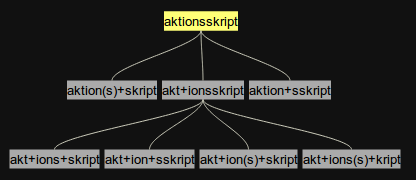
\includegraphics{images/tree.png}
  \end{center}
  \caption{Visualized split of the word \emph{aktionsskript}}
  \label{img_tree}
\end{figure}

\subsubsection{Data driven algorithm}

As alternative to the left to right splitting algorithm a complete other algorithm was implemented. This algorithm is more data focused. It tries to split the word based on the amount of words that begin and end with the same letters as the word that should be splitted. This idea was first tried by Larson \cite{dd}.

To split a word the IGerman98 dictionary was packed in a Trie (\url{http://en.wikipedia.org/wiki/Trie}). The trie can now return a number words that begin with the same letters. For example if the trie contains \emph{abc}, \emph{abcde} and \emph{abde} the value of \emph{a} is three, because three words start with \emph{a}, the value for \emph{abd} is \emph{1} because one word starts with this letters. An additional trie is computed with all words in reserve (\emph{abc} -> \emph{cba}). With both tries generated the main algorithm can now start. The next three tables~\ref{ex_dd_1}~,~\ref{ex_dd_2}~and~\ref{ex_dd_2} show an example (extracted from \cite{dd}).

\begin{table}[h]
\begin{center}
  \begin{tabular}{|l|l|l|l|l|l|l|l|l|l|l|l|l|l|l|l|}
    \hline
    f&r&i&e&d&e&n&s&p&o&l&i&t&i&k \\ \hline
    -&-&39&29&29&25&24&23&3&1&1&1&1&1&1 \\ \hline
    1&1&1&1&1&2&7&37&88&89&89&92&99&-&- \\ \hline
  \end{tabular}
  \caption{First extract the trie values for each part. We define that a word has at least three letters.}
  \label{ex_dd_1}
\end{center}
\end{table}

\begin{table}[h]
\begin{center}
  \begin{tabular}{|l|l|l|l|l|l|l|l|l|l|l|l|l|l|l|l|}
    \hline
    f&r&i&e&d&e&n&s&p&o&l&i&t&i&k \\ \hline
    -&-&-&10&0&4&1&1&20&2&0&0&0&0&0 \\ \hline
    0&0&0&0&0&5&30&51&1&0&3&7&-&-&- \\ \hline
  \end{tabular}
  \caption{Next we calculated the difference of the neighbors.}
  \label{ex_dd_2}
\end{center}
\end{table}

\begin{table}[h]
\begin{center}
  \begin{tabular}{|l|l|l|l|l|l|l|l|l|l|l|l|l|l|l|l|}
    \hline
    f&r&i&e&d&e&n&s&p&o&l&i&t&i&k \\ \hline
    -&-&-&-& &*& & &*& & & & & &  \\ \hline
     & & & & & & &*& & & &-&-&-&- \\ \hline
  \end{tabular}
  \caption{Local maxims are possible splitting points (marked with a asterisks)}
  \label{ex_dd_3}
\end{center}
\end{table}

For this example the split is made between \emph{friedens} and \emph{politik}; which are correct words. The splitting can be done recursively on each part again until nothing can be splitted anymore. The evaluation for this algorithm works exactly like the evaluation of the left to right algorithm and can be seen in table~\ref{tab_eval_dd}.

\begin{table}[h]
  \begin{center}
    \begin{tabular}{l | l | l}
      \hline
      \textbf{Algorithm}  & \textbf{Correct with morphemes} & \textbf{Correct without morphemes} \\ \hline
      Data driven & 0.16 & 0.41 \\ \hline
    \end{tabular}
  \end{center}
  \caption{Evaluation result data driven splitting algorithm}
  \label{tab_eval_dd}
\end{table}

As we can see the result of this algorithm are not very good compared to the left to right splitting algorithm. It is nearly impossible to use this splitting for the ranking algorithm. But that do not mean that this algorithm is always bad. Depending on your dataset or with another dictionary this can be a helpful alternative.

\subsubsection{Conclusion}

In the above sections we developed two complete different splitting algorithm. While the left to right algorithm splits a word if a subpart of the word is in the dictionary, the data driven algorithm tries to extract some statistics from the dictionary to find a more natural split. For the current dataset the left to right splitting algorithm works a lot better. The further work only based on this algorithm. But for special dataset the data driven algorithm can be a good alternative.

\begin{table}[h]
\begin{center}
\begin{tabular}{l | l | l}
  \hline
  \textbf{Algorithm}  & \textbf{Correct with morphemes} & \textbf{Correct without morphemes} \\ \hline
  Left to right & 0.81 & 0.89 \\ \hline
  Data driven & 0.16 & 0.41 \\ \hline
\end{tabular}
\end{center}
\caption{Results of splitting algorithm}
\end{table}

\subsection{Ranking algorithms}

With the splitting algorithm we are able to create a lot of possible splits for a word. The ranking algorithm now tries to order these splits. The splits with the highest value will be the correct split. The list of possible splits contains also the inital word. If the initial word gets the highest rank no splitting is done.

All three ranking algorithm have to methods of ranking. They can rank a list or rank a tree. Ranking on a list gives all possible splits a weight, while ranking on a tree gives only a subset of all possible splits a weight:

\begin{lstlisting}
function listRanking(list)
  result = List()
  for each (item in list)
    result += rank(item)
  result.order()

  return result(0)


function treeRanking(parent)
  if (parent.isLeaf())
    return parent

  list = parent + parent.children()
  res = listRanking(list)

  if (res == parent)
    return parent
  else
   treeRanking(res)
\end{lstlisting}

The evaluation of each algorithm checks if the highest ranked value is the correct split. As in the splitting algorithm evaluation we also distinguish between correct with morphemes and correct without morphemes. For the list ranking we also check how many correct results are in the first two and three elements of the ranked list. We call this \emph{Correct@1}, \emph{Correct@2} and \emph{Correct@3}. We must also keep in mind that we can have a maximum of 0.81 with morphemes and 0.89 without morphemes due to the splitting algorithm.

The evaluation of the ranking algorithm was done only on a small subset of examples (10,000), because the Lucene index was very slow. The result of the splitting algorithm on these dataset is the following:

\begin{table}[h]
\begin{center}
\begin{tabular}{l | l | l}
  \hline
  \textbf{Algorithm}  & \textbf{Correct with morphemes} & \textbf{Correct without morphemes} \\ \hline
  Left to right & 0.813 & 0.888 \\ \hline
\end{tabular}
\end{center}
\caption{Left to right splitting evaluation on the dataset of 10,000 elements}
\end{table}

\subsubsection{Frequency based ranking}
The first attempt to build a ranking function is a frequency based method as described by Alfonseca \cite{alf2008}. For each split $S$ with the words $s_i$ we calculate the geometric mean of the frequencies from the \texttt{Web1T} corpus:

\begin{equation}
  F_s = \prod_{s_i \in S} freq(s_i))^{\frac{1}{|S|}}
\end{equation}

The \texttt{freq} value is calculated with the \texttt{Finder} class. This class contains the method \texttt{find} which returns a list of n-grams that match the search word. For each n-gram we also get the frequency. The result of \texttt{freq} is the sum of all frequencies in the list. The split with the highest $F_s$ will be the highest ranked split.

For the evaluation the command line tool in \texttt{bin/frequencyBased.sh} can be used. It can have following parameter:

\begin{lstlisting}
usage: FrequencyBasedRanker
    --limit <arg>         (optional) Limit of results to evaluate
    --luceneIndex <arg>   The path to the web1t lucene index
\end{lstlisting}

The current evaluation is only done on 10,000 example as mentioned above. For that we can set the \texttt{limit} parameter to 10,000. The \texttt{luceneIndex} parameter is required and has as argument the path to the generated lucene index. The evaluation of the algorithm is show in table~\ref{eval_freq}. The values in brackets are the correct results without morphemes.

\begin{table}[h]
  \begin{center}
    \begin{tabular}{|l|l||l|l|l|}
      \hline
      \textbf{Algorithm} & \textbf{Correct tree} & \textbf{Correct@1} & \textbf{Correct@2} & \textbf{Correct@3} \\ \hline
      Frequency based & 0.5226  (0.7204) & 0.5078 (0.7029) & 0.6653 (0.7847) & 0.7263 (0.8291) \\ \hline
    \end{tabular}
  \end{center}
  \caption{Evaluation results for the frequency based algorithm}
  \label{eval_freq}
\end{table}

As we can see, the result without morphemes are a lot better than the result with morphemes. When we are not interested in morphemes the tree gives us with 0.7204 correct answers the best results but the list with 0.7029 is not far behind. We also can see the increase from Correct@1 to Correct@3 is not the same for the value with/without morphemes. The correct answers with morphemes increase from 0.578 to 0.7263. That is a difference of 0,2185. The differences for the correct without morphemes is only $0.8291-0.7029 = 0.1262$. That means that the results at the second or third place often only differ in the position of the morphemes, but not at the split positions.

\subsubsection{Probability based ranking}
The second method is also described by Alfonseca \cite{alf2008}. For each Split $S$ with the words $s_i$ we calculate

\begin{equation}
  P_s = \sum_{s_i \in S} -log(\frac{freq(s_i)}{F})
\end{equation}

where $F$ is the total amount of frequencies. The split with the lowest $P_s$ will be the highest ranked split.

For the calculation of $F$ the command line tool in \texttt{bin/countTotalFreq} can be used with the following options:

\begin{lstlisting}
usage: countTotalFreq
    --index    The path to the web1t lucene index
\end{lstlisting}

The result is the sum of all frequency values in the Lucene index. This value must be set in the property file \texttt{src/main/resources/index.properties} with the property name \texttt{frequency}. Example:

\begin{lstlisting}
# src/main/resources/index.properties
frequency = 143782944956
\end{lstlisting}

As you can see the value can be bigger than the Integer range. In the implementation Java's \texttt{BigInteger} class is used.

After setting up the $F$ value the evaluation can be started from the command line (\texttt{bin/probabilityBased.sh}). It has the same parameter as the command line tool for the Frequency based algorithm. The evaluation on 10,000 examples returns the result shown in table~\ref{eval_prob}.

\begin{table}[h]
  \begin{center}
    \begin{tabular}{|l|l||l|l|l|}
      \hline
      \textbf{Algorithm} & \textbf{Correct tree} & \textbf{Correct@1} & \textbf{Correct@2} & \textbf{Correct@3} \\ \hline
      Probability based & 0.1815  (0.2518) & 0.1843 (0.2558) & 0.5095 (0.6579) & 0.6281 (0.7425) \\ \hline
    \end{tabular}
  \end{center}
  \caption{Evaluation results for the probability based algorithm}
  \label{eval_prob}
\end{table}

The result are not very good compared to the result of the frequency based method. Both tree and list ranking return only a success rate of 0.18 with morphemes and 0.25 without morphemes. But I we look at the \emph{Correct@2} and \emph{Correct@3} values we see a great increase. This function favors split with a small amount of total split. Here, words with no split or one split will be higher ranked than words with three or four splits. That means the result of this algorithm ca be a good feature for a machine learning algorithm, were several algorithm are combined. 

\subsubsection{Mutual information based ranking}
The previous methods only focus on the individual words and not on the co-occurrence of the words. For that we add the next method, also described by Alfonseca \cite{alf2008}. For a word pair $w_1$ and $w_2$ we can calculate the mutual information:

\begin{equation}
  M(w_1, w_2) = log_2(\frac{\frac{freq(w_1, w_2)}{F}}
    {\frac{freq(w_1)}{F} \times \frac{freq(w_2)}{F}})
    = log_2(\frac{F \times freq(w_1, w_2)}{freq(w_1) \times freq(w_2)})
\end{equation}

For all word pairs in a split $S$ we can calculate the mutual information and average it. The split with the highest averaged mutual information is the highest ranked split.

Before we can start the evaluation we have to set the $F$ value as the the previous section described. To start the evaluation again the command line tool in \texttt{bin/mutualInformationBased.sh} can be used. It has the same parameter as the command line tool for the frequency based evaluation. The results are shown in table~\ref{eval_mutual}

\begin{table}[h]
  \begin{center}
    \begin{tabular}{|l|l||l|l|l|}
      \hline
      \textbf{Algorithm} & \textbf{Correct tree} & \textbf{Correct@1} & \textbf{Correct@2} & \textbf{Correct@3} \\ \hline
      Mutual information based & 0.2952 (0.4415) & 0.3681 (0.5420) & 0.5163 (0.6659) & 0.5865 (0.7371) \\ \hline
    \end{tabular}
  \end{center}
  \caption{Evaluation results for the mutual information based algorithm}
  \label{eval_mutual}
\end{table}

The results of the mutual information based algorithm are a little bit better than the result of the probability based method but not as good as the frequency based method. Also the increase of the \emph{Correct@2} and \emph{Correct@3} values is not so high as in the probability based method.

\subsubsection{Conclusion}

In total the frequency based algorithm was the best ranking algorithm of all three. The success rate of 72\% is not far away from the maximum of 88\%. Improving the splitting algorithm can also improve the ranking algorithm. The other two ranking algorithm do not return useful results, but they can be used in combination with some other algorithm in a machine learning based ranking algorithm. Due to a time limit this was not implemented. But the work of  Alfonseca \cite{alf2008} showed good results.

A current problem for all algorithms is that the time to access the index is very long. This caused the problem that not the complete dataset could be evaluated. Improving the index or using faster hardware is a must for all \emph{real world} problems.

\begin{table}[h]
  \begin{center}
    \begin{tabular}{|l|l||l|l|l|}
      \hline
      \textbf{Algorithm} & \textbf{Correct tree} & \textbf{Correct@1} & \textbf{Correct@2} & \textbf{Correct@3} \\ \hline
     Frequency based & 0.5226  (0.7204) & 0.5078 (0.7029) & 0.6653 (0.7847) & 0.7263 (0.8291) \\ \hline
      Probability based & 0.1815  (0.2518) & 0.1843 (0.2558) & 0.5095 (0.6579) & 0.6281 (0.7425) \\ \hline
      Mutual information based & 0.2952 (0.4415) & 0.3681 (0.5420) & 0.5163 (0.6659) & 0.5865 (0.7371) \\ \hline
    \end{tabular}
  \end{center}
  \caption{Results of ranking algorithms}
\end{table}

\subsection{UimaFit Component}

To bring the splitting and ranking algorithm together a Uima Compoenent was implemented with the help of the UimaFit library. The component has two Annotator, one for the list based ranking, called \texttt{NounDecompoundingListAnnotator} and one for the tree based ranking, called \texttt{NounDecompoundingTreeAnnotator}. Both work very similar, with the difference than one called the tree ranking function and the other the list ranking function.

Before using the component in a analysis engine a tokenizer is needed that creates token annotations on the document. After the tokenizer annotator one of the two above mentioned annotators can be used. Both components have three configuration parameter. With the \texttt{index} parameter the path to the lucene index must be set. The \texttt{tokenClassName} parameter contains the classname of the token annotation created by a tokenizer. The last and optional parameter is the \texttt{ranker} parameter. Here you can set with ranking algorithm you want to use. Default is \texttt{FREQUECNY}. Both algorithm use the left to right splitting algorithm with the IGerman98 dictionary.

After processing the annotator on a document a new annotation type is added to the document. For each token the \texttt{SplittedToken} type is added. It covers the same text as the token and has as additional information a list of splits elements. Each element can have brackets to identify morphemes. Concatenating the split elements will return the original token.

\chapter{Reflection}

\subsection{Lessons Learned}

\subsubsection{Time management}

Weekly time planning help me to think about the goals for the next week. Most of the time I planned the amount of time correctly or I needed less time. I never came to the point that I planned the time totally wrong. Because of that I think I can understand the complexity of the problems that need to be solve and my own skills of implementation.

Appreciating the time work very good, but doing the things on the day I planned worked not so good. Often I reorganized the day-planning in a week. Most of the time this happened because other work was not done or I don't feel like it. But the efficiency is much higher on the days when I feel very well.

\subsubsection{Weekly documentation}

Next to the time management also the weekly documentation helped me to get an overview of the next steps and the total project. It was also a very good help to write this report. Some ideas that failed during the project get forgotten very fast. Writing them done in the weekly documentation and the final report, prevents other to do the same mistakes.

Having deadlines for the weekly documentation also helps to reach the goals planned in the current week.

\subsection{Conclusion}

Noun compounding in the German language is a powerful tool to build new words with two or more existing words. The meaning of the new word is not total different. The single words can stand in the same context as the compound word. This is a problem in many NLP task. Search engine for example have to search for the compound and the splitted words to find all relevant examples.

In this work we saw some method to split compound words into base words. In general we take a compound word and try to generate lots of possible splits with the help of a dictionary. Afterwards we rank each split. The split with the highest value is our splitted compound.

To generate possible split we saw two different techniques. The left to right algorithm works best and returns with a rate of 81\% a list that contains the correct split. This algorithm can also return a tree instead of list, which gives us the possibility to visualizes the algorithm. We can also use this tree in the ranking function to minimize the calculations.

After developing a successful splitting algorithm, we focus on the ranking algorithms. The base idea for all three developed solution was that splits with more relevant words are correct. This knowledge of what are relevant word comes from the Google Web1T corpus. At the end the frequency based algorithm works best. With a success rate of 72\% (without morphemes) we get some useful results. The other two algorithm do not return useful results, but they can be used as features for a machine learning algorithm. Combining all three algorithm in a machine learning algorithm can improve the result, but was not done in this work.

A currently unsolved problem is that splitting a word takes very long because the Lucene index is very slow. Faster hardware can help to resolve this problem, but was not tested.

At the end we have a useful result that can be used in a NLP Task, in form of a Uima component.

\appendix

\chapter{Appendix}

\section{Installation of the visualization tool}

The left to right algorithm has simple tool to visualize the splits in a tree. This section shows you how to install this app.

At first need to install all required software.

\textbf{Warning:} CouchDB will be merged with Membase in future. This installation will work with CouchDB 1.0.0+

\begin{enumerate}
  \item Install \texttt{couchdb} from \url{http://www.couchone.com/get} or install the package \texttt{couchdb} on Ubuntu
  \item Install \texttt{node.js} from \url{http://nodejs.org/} (tested with version 0.2.3).
  \item Install \texttt{npm} (Node package manager) as descripted on \url{http://npmjs.org/}
  \item Install \texttt{node.couchapp.js} from \url{https://github.com/mikeal/node.couchapp.js}. See the readme file for more information. This project should also work with newer version of \texttt{node.js}.
\end{enumerate}

After all required software is install we can upload the application to \texttt{couchdb}. For that we use \texttt{node.couchapp.js}.

\begin{enumerate}
  \item Open a browser and open \url{http://localhost:5984/_utils/}.
  \item Create a database with some name (e.g. ``noun\_decompound'')
  \item Open a terminal a change to the directiory \texttt{src/main/couchapp}
  \item Execute \texttt{couchapp push app.js http://localhost:5984/dbname}. Change \texttt{dbname} to what you set in step two.
  \item Your application should now run under \url{http://127.0.0.1:5984/dbname/_design/tree/index.html}. But the database contains now data.
\end{enumerate}

The last step is to update some data to the database.

\begin{enumerate}
  \item Open a terminal a change the directory to the project
  \item Execute \texttt{./bin/couchDbExport.sh --limit 20000 --dbname=dbname}. This will generate 20,000 splits an saves them to the database.
  \item Reload your the application in the browser. On the left side all generated split should appear. Click on them to see the tree. Have fun!
\end{enumerate}

During the project I uploaded the app to \url{http://jenshaase.couchone.com/noun_decompounding/_design/tree/index.html}. Use the link to see how should look like.

\bibliographystyle{alpha}
\bibliography{11_finalReport}

\end{document}
